\documentclass{article}
\usepackage{graphics}
\usepackage{indentfirst}
\usepackage{amsmath}
\usepackage{algorithm}
\usepackage{algorithmic}
\usepackage{bm}
\usepackage{setspace}
\usepackage{graphicx}
\usepackage{float}
\usepackage{CJKutf8}



\title{分布式机器学习笔记}
\author{Ruichen Wang}

\begin{document}
\begin{CJK*}{UTF8}{gbsn}
\maketitle
\begin{abstract}
---
\end{abstract}

\tableofcontents
\section{基本知识}
Communication Backends 主要有四种:
\begin{itemize}
\item TCP 
\begin{itemize}
\item 适用范围广,大部分系统和机器都提供支持。支持cpu上的p2p和collective functions。但是不支持GPU,优化程度也不高。
\end{itemize}
\item MPI
\item Gloo
\item NCCL
\end{itemize}

\begin{figure}[H]
\centering
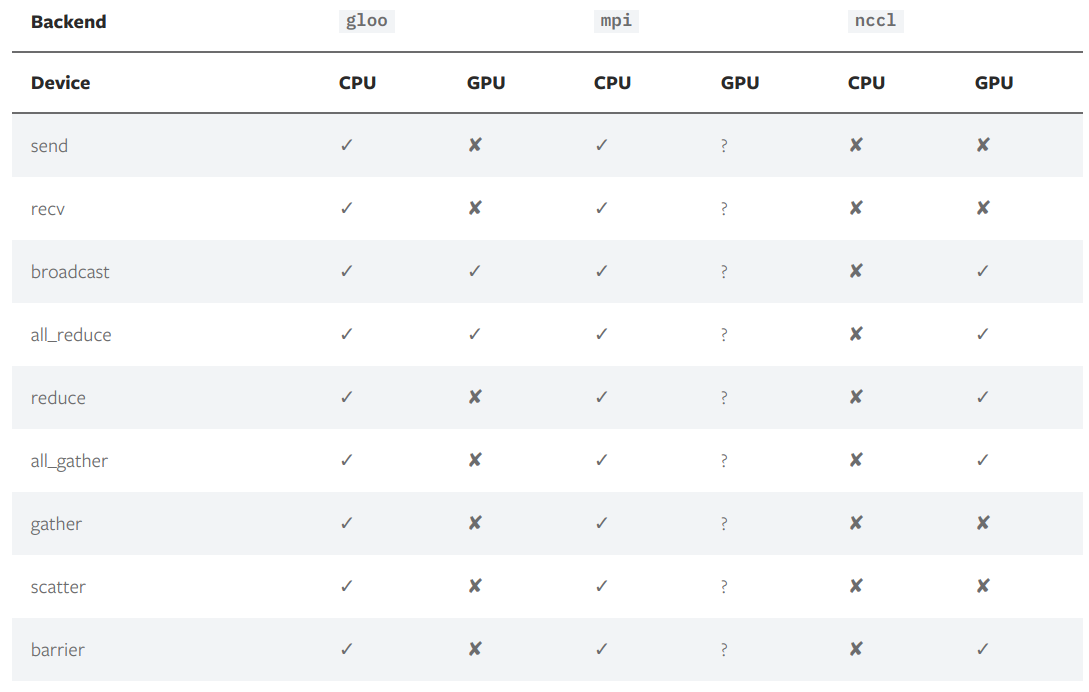
\includegraphics[width=5in,height=3in]{backends}
\caption{backends}
\end{figure}




\end{CJK*}
\end{document}




















